\section{Capítulo: Diseño}

En este capítulo se presenta el diseño detallado de los módulos
que constituyen el sistema para el monitoreo de la
fermentación en tiempo real. Se abordan la
arquitectura general, los diagramas y la topología de
comunicación entre dispositivos y servicios en la nube. Se
detallan el diseño de cada componente previamente seleccionado en 
el capítulo \ref{sec:cap5}
,como
Python 
para el análisis de datos, MongoDB para el almacenamiento de documentos
JSON, React y React-Chartjs-2 para la visualización en tiempo
real, microcontroladores XIAO ESP32 para adquisición de datos y
EMQX Cloud como broker MQTT— así como la propuesta de despliegue
en AWS para asegurar escalabilidad y disponibilidad.
\newline
\newline
El diseño cubre los Módulos 1 a 4 jutno con el diseño del broker MQTT y el
servidor, en donde se especifica la estructura de
la base de datos, los formatos de mensajes MQTT, 
las interfaces de usuario y las consideraciones de
seguridad y rendimiento.Con el fin de cumplir con los requisitos
funcionales  y los no funcionales relativos a escalabilidad, flexibilidad ante cambios en
los esquemas de datos y baja latencia en la comunicación. A lo
largo del capítulo se incluyen diagramas lógicos, esquemas de
colecciones y ejemplos de payloads JSON que facilitarán la
implementación y validación.

\subsection{Diseño Módulo 1}
En esta sección se describen e ilustra los diagramas necesarios para llevar a 
cabo el funcionamiento de dicho módulo, así como la descripción 
detallada de cada uno de ellos, proporcionando la secuencia de operación del módulo y
el diseño del circuito integrando todos los componentes previamente seleccionados en 
la sección \ref{sec:mod1}, 
aparte se detalla un módelo 3D de los frascos  integrando los sensores y el microcontrolor. 

\subsubsection{Diagrama Módulo 1}
Como primera parte se define el diagrama del módulo 1, tal como se aprecia en la \cref{fig:Flu1}.  
En dicha figura se ilustra el flujo qeu seguira el microcontrolador, desde la verificación de la conexión MQTT 
hasta el envío de datos y la gestión de alarmas, por lo que cada decisión y acción se traduce en una cadena JSON 
específica que viaja al broker EMQX Cloud.  
A continuación se describen las tres alarmas críticas, junto con la cadena exacta que publica el microcontrolador al broker:

\begin{enumerate}
    \item \textbf{Alarma 1:} Se activa cuando cualquier sensor falla ya sea en modo monitoreo o prueba, generando la cadena siguiente cadena "Fallo sensor pH/CO2/temperaturaesté".
    \item \textbf{Alarma 2:} Se activa cuando el microcontrolador esta en modo monitoreo y detectan que los datos iniciales estan fuera de rango, generando la siguiente cadena "Condiciones iniciales fuera de rango"+"pH"+"Temperatura"
    \item \textbf{Alarma 3:} Se activa cuando el microcontrolador en modo monitoreo detecta que el pH supero el limite de 3.9, generando una cadena "pH fuera de rango"+"pH"
    \item \textbf{Alarma 4:} Se activa cuando el usuario desea terminar el proceso de monitoreo, generando una cadena "Fin de la fermentación"
\end{enumerate}

\begin{figure}[htb]
    \centering
    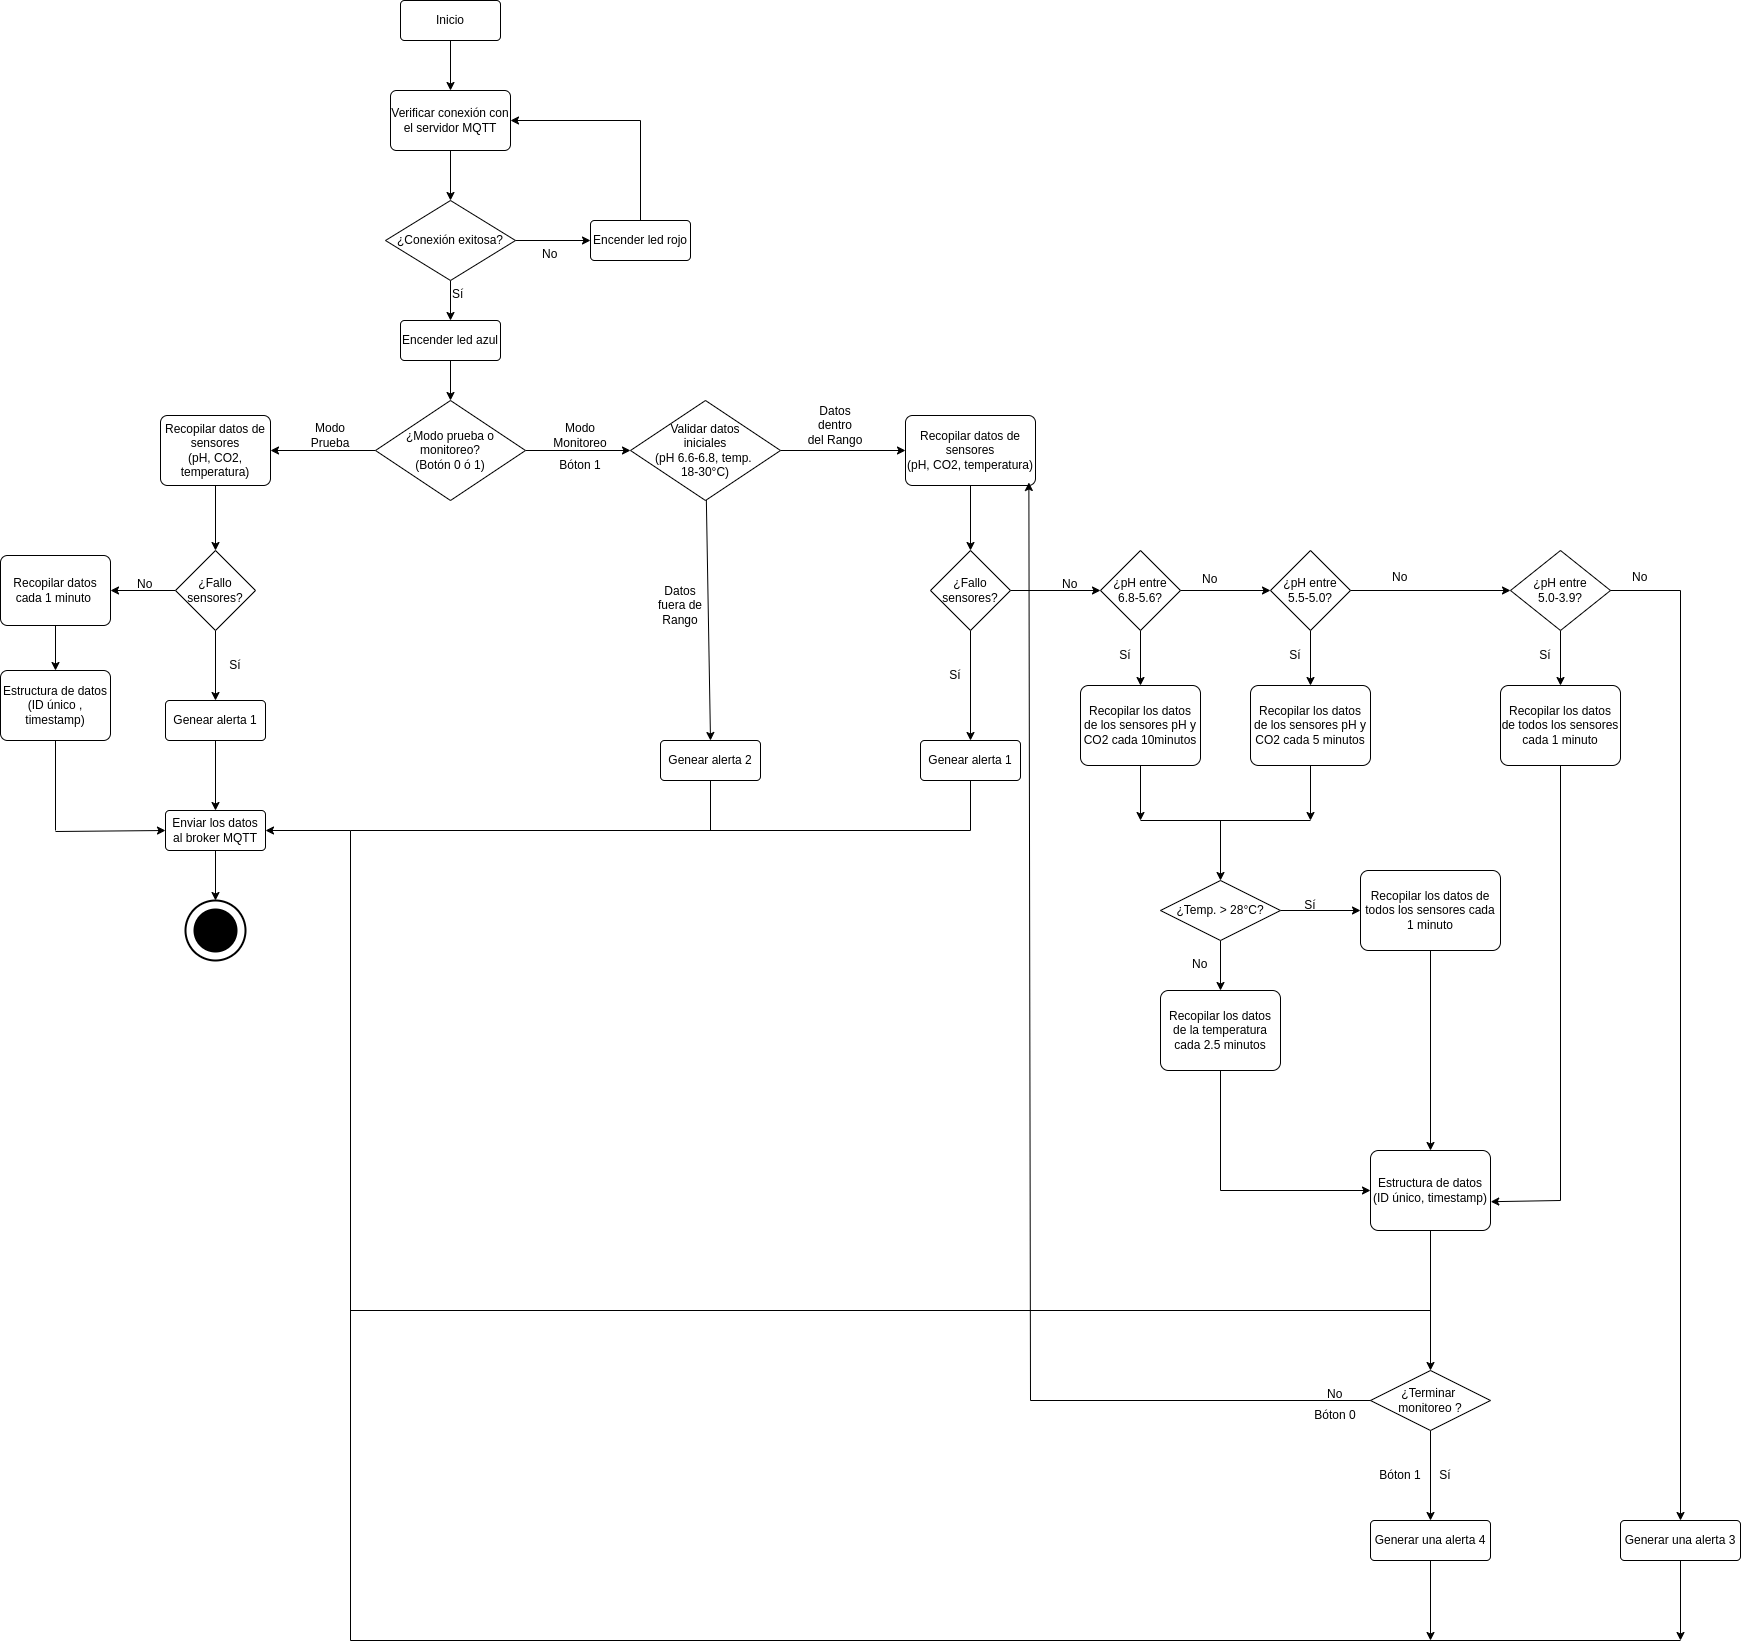
\includegraphics[
        width=1\textwidth,        % Máximo ancho del texto disponible
        height=1\textheight,  % Máximo alto del texto (usamos 95% para dejar espacio al pie)
        keepaspectratio          % Mantiene las proporciones originales
    ]{./UML/Modulo1/Diseno/diagrama.drawio.png}
    \caption{Diagrama del módulo 1}
    \label{fig:Flu1}
\end{figure}


